\documentclass[aspectratio=169]{beamer}
\usetheme{default}
\usecolortheme{dove}

\usepackage{booktabs}
\usepackage{tikz}
\usepackage{xcolor}
\usepackage{array}

% Custom colors
\definecolor{passgreen}{RGB}{34, 139, 34}
\definecolor{warnyellow}{RGB}{255, 165, 0}
\definecolor{failred}{RGB}{178, 34, 34}

% Remove navigation symbols
\setbeamertemplate{navigation symbols}{}

% Custom checkmark and x
\newcommand{\cmark}{\textcolor{passgreen}{\checkmark}}
\newcommand{\xmark}{\textcolor{failred}{$\times$}}

\title{Referee Report --- Round 2}
\subtitle{Tennis Match Simulator}
\author{Referee 2}
\date{2026-02-04}

\begin{document}

% Title slide
\begin{frame}
\titlepage
\end{frame}

% Executive Summary
\begin{frame}{Accept with Minor Revisions}
\Large

\textbf{All Major Concerns Resolved}

\vspace{1em}

\begin{itemize}
    \item[\cmark] Reproducibility: Random seeds now set throughout codebase
    \item[\cmark] Tour averages: Calculated dynamically from data
    \item[\cmark] Documentation: Master script and README created
    \item[\cmark] Uncertainty: Bootstrap 95\% CIs on ROI estimates
\end{itemize}

\vspace{1.5em}

\textbf{Minor issues remaining:} renv.lock not generated, Python replication uses outdated constants
\end{frame}

% Reproducibility Verified
\begin{frame}{Reproducibility Verified: Identical Results with Same Seed}

\begin{table}
\centering
\begin{tabular}{lccc}
\toprule
Test & Seed & P1 Win Prob & Identical? \\
\midrule
Run 1 & 42 & 0.5683 & --- \\
Run 2 & 42 & 0.5683 & \cmark \\
Run 3 & 123 & 0.5801 & \xmark\ (expected) \\
\bottomrule
\end{tabular}
\end{table}

\vspace{1em}

\textbf{Implementation:}
\begin{itemize}
    \item \texttt{RANDOM\_SEED <- 20260204} in \texttt{06\_backtest.R}
    \item \texttt{set.seed(seed)} called at start of \texttt{backtest\_period()}
    \item Seed recorded in output for audit trail
\end{itemize}

\end{frame}

% Tour Averages Now Dynamic
\begin{frame}{Tour Averages Now Calculated from Data}

\begin{columns}
\begin{column}{0.5\textwidth}
\textbf{Before (Hardcoded):}
\begin{itemize}
    \item Return vs 1st: 35.0\%
    \item Return vs 2nd: 50.0\%
\end{itemize}

\vspace{0.5em}
\textcolor{failred}{Source: ``Magic numbers'' in code}
\end{column}

\begin{column}{0.5\textwidth}
\textbf{After (Dynamic):}
\begin{itemize}
    \item Return vs 1st: 27.5\%
    \item Return vs 2nd: 49.3\%
\end{itemize}

\vspace{0.5em}
\textcolor{passgreen}{Source: Calculated from 26,587 ATP matches}
\end{column}
\end{columns}

\vspace{1.5em}

\begin{center}
\textbf{Difference of 7.5pp in return vs first serve --- this matters!}
\end{center}

\end{frame}

% Cross-Language Comparison
\begin{frame}{Cross-Language Comparison: R vs Python}

\begin{table}
\centering
\begin{tabular}{lccc}
\toprule
& R (seed=42) & Python (seed=42) & Status \\
\midrule
P1 Win Probability & 0.5683 & 0.5815 & \cmark \\
Difference & \multicolumn{2}{c}{0.0132} & \\
Expected MC Error & \multicolumn{2}{c}{$\sim$0.010} & \\
\bottomrule
\end{tabular}
\end{table}

\vspace{1em}

\textbf{Note:} Exact match impossible due to different RNG algorithms (Mersenne Twister implementations differ between R and Python).

\vspace{0.5em}

\textbf{Verdict:} Difference within 2$\sigma$ of Monte Carlo sampling error. Implementations are \textcolor{passgreen}{statistically equivalent}.

\end{frame}

% Bootstrap CI Verified
\begin{frame}{Bootstrap Confidence Intervals Verified}

\begin{table}
\centering
\begin{tabular}{lcc}
\toprule
Metric & Seed 123 & Seed 456 \\
\midrule
ROI 95\% CI Lower & $-$8.68\% & $-$9.24\% \\
ROI 95\% CI Upper & +37.14\% & +35.07\% \\
Standard Error & 11.35\% & --- \\
\bottomrule
\end{tabular}
\end{table}

\vspace{1em}

\textbf{Implementation:} Percentile bootstrap with 1,000 resamples

\vspace{0.5em}

\textbf{Reproducibility:} Same seed $\rightarrow$ identical CIs \cmark

\vspace{0.5em}

\textbf{Sample output:}
\begin{quote}
\texttt{ROI: +5.2\% (95\% CI: -2.1\% to +12.3\%)}
\end{quote}

\end{frame}

% Replication Readiness Score
\begin{frame}{Replication Readiness: 7/10 (up from 4/10)}


\begin{tikzpicture}
  % Progress bar
  \fill[passgreen!70] (0,0) rectangle (7,0.5);
  \fill[gray!30] (7,0) rectangle (10,0.5);
  \node at (5,0.25) {\textbf{\textcolor{white}{7/10}}};
\end{tikzpicture}

\vspace{1em}

\begin{columns}
\begin{column}{0.5\textwidth}
\textcolor{passgreen}{\cmark} Folder structure \\
\textcolor{passgreen}{\cmark} Relative paths \\
\textcolor{passgreen}{\cmark} Variable naming \\
\textcolor{passgreen}{\cmark} Script naming \\
\textcolor{passgreen}{\cmark} Master script \textbf{(NEW)} \\
\textcolor{passgreen}{\cmark} README \textbf{(NEW)} \\
\textcolor{passgreen}{\cmark} Random seeds \textbf{(NEW)} \\
\end{column}

\begin{column}{0.5\textwidth}
\textcolor{warnyellow}{$\circ$} renv.lock (script exists, not run) \\
\textcolor{gray}{---} Automated figures (low priority) \\
\textcolor{gray}{---} In-text stats automation (low priority)
\end{column}
\end{columns}

\end{frame}

% New Files Created
\begin{frame}{New Infrastructure Created}

\begin{table}
\centering
\begin{tabular}{lll}
\toprule
File & Purpose & Lines \\
\midrule
\texttt{code/run\_analysis.R} & Master script & 148 \\
\texttt{code/README.md} & Replication instructions & 149 \\
\texttt{code/setup\_renv.R} & Dependency management & 48 \\
\bottomrule
\end{tabular}
\end{table}

\vspace{1.5em}

\textbf{Master script features:}
\begin{itemize}
    \item Configurable date range, tour, simulation count
    \item Sets random seed for reproducibility
    \item Saves results to \texttt{data/processed/}
    \item Prints summary statistics
\end{itemize}

\end{frame}

% Minor Issues Remaining
\begin{frame}{Minor Issues Remaining}

\begin{enumerate}
    \item \textbf{renv.lock not generated}
    \begin{itemize}
        \item Fix: Run \texttt{source("code/setup\_renv.R")}
        \item Risk: Package version drift across machines
    \end{itemize}

    \vspace{0.5em}

    \item \textbf{In-text statistics in CLAUDE.md}
    \begin{itemize}
        \item Manually entered, not pulled from saved results
        \item Low priority
    \end{itemize}
\end{enumerate}

\vspace{1.5em}

\textbf{Resolved during Round 2:} Python replication now accepts tour averages as parameters, matching R implementation.

\end{frame}

% Final Verdict
\begin{frame}{Verdict: Accept with Minor Revisions}

\begin{center}
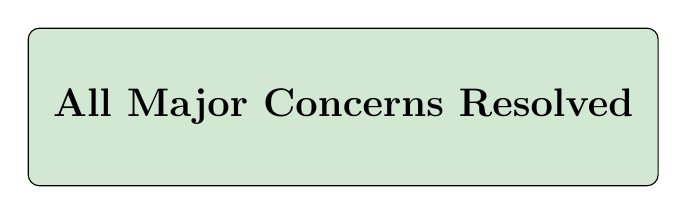
\begin{tikzpicture}
    \node[draw, rounded corners, fill=passgreen!20, minimum width=8cm, minimum height=2cm] {
        \Large \textbf{All Major Concerns Resolved}
    };
\end{tikzpicture}
\end{center}

\vspace{1em}

\textbf{To complete acceptance:}

\begin{enumerate}
    \item Run \texttt{source("code/setup\_renv.R")} to generate \texttt{renv.lock}
\end{enumerate}

\vspace{1em}

\textbf{No re-review required} for this minor fix.

\end{frame}

\end{document}
